% GUIDING QUESTIONS:
%
% What are the key artifacts of your project (e.g., methodology, hardware
% design, software algorithm, optimization or control technique)?
%
% How are these artifacts implemented and evaluated?
%
% What are your most important empirical or theoretical results?

\begin{frame}{Results}
    \huge
    \centering
    Results
\end{frame}

\begin{frame}{Simulating}
    \begin{columns}
        \column{0.5\textwidth}
        \begin{itemize}
            \item Created a simulation program using symbolic expression library
                  \texttt{symengine.py} \cite{symengine}
            \item Ran 20 simulations for varying $n$, $m$ using random initial conditions
            \item Pursuers strictly faster than evaders, and evaders following random walk
            \item Wrote data analysis script \& a C visualization engine \cite{diffgames}
        \end{itemize}

        \column{0.5\textwidth}
        \begin{figure}
            \centering
            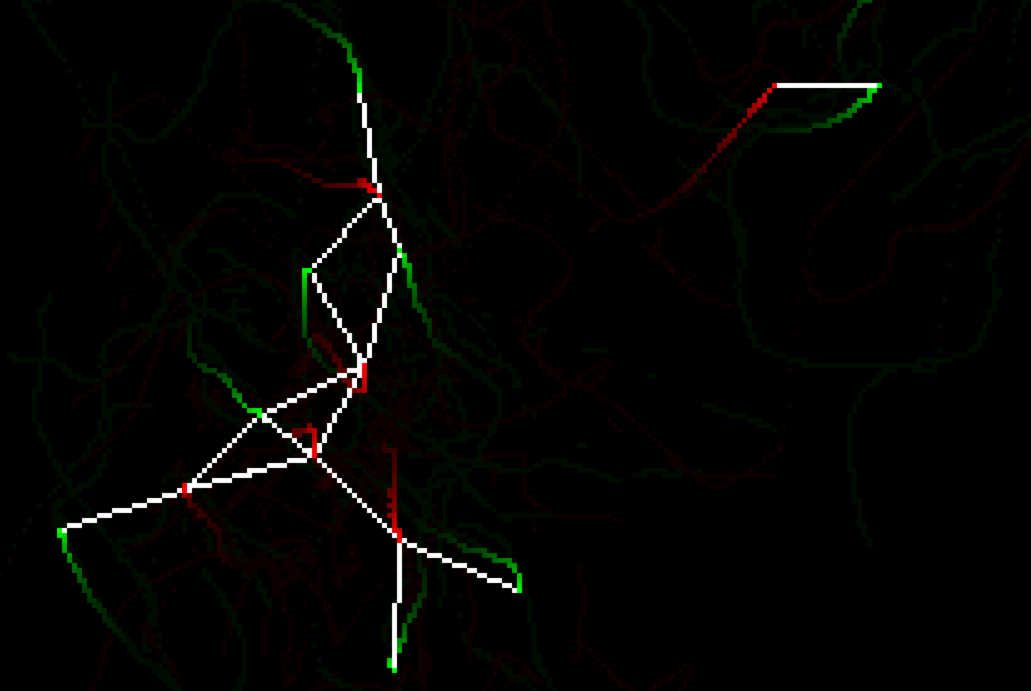
\includegraphics[width=0.75\linewidth]{assets/n10m10_graph.png}
            \caption{Interesting network formation with $n = m = 10$}
        \end{figure}
    \end{columns}
\end{frame}

% TODO: include videos of these?

\begin{frame}{$m = 2$ chains}
    \begin{figure}
        \subfloat[Random initial positions]{
            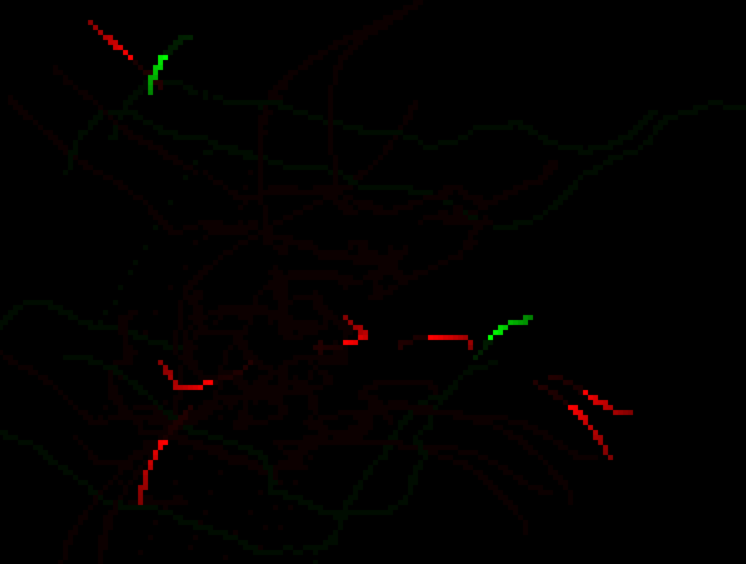
\includegraphics[width=0.4\textwidth]{assets/n8m2_initial_pos.png}
        }
        \subfloat[Chain formation connecting all agents]{
            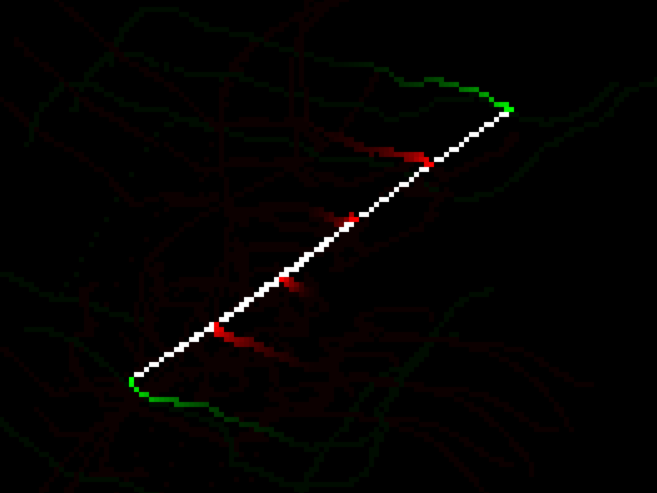
\includegraphics[width=0.4\textwidth]{assets/n8m2_chain.png}
        }
        \caption{Simulations with $m = 2$ form a chain for optimal connectivity (pictured $n = 8$)}
    \end{figure}
    {\tiny Pursuers in red, evaders in green, connections in white.
    Visualization from a bird's eye view.}
\end{frame}

\begin{frame}{Pursuer grouping for large $n$}
    \begin{figure}
        \subfloat[Random initial positions converging to group]{
            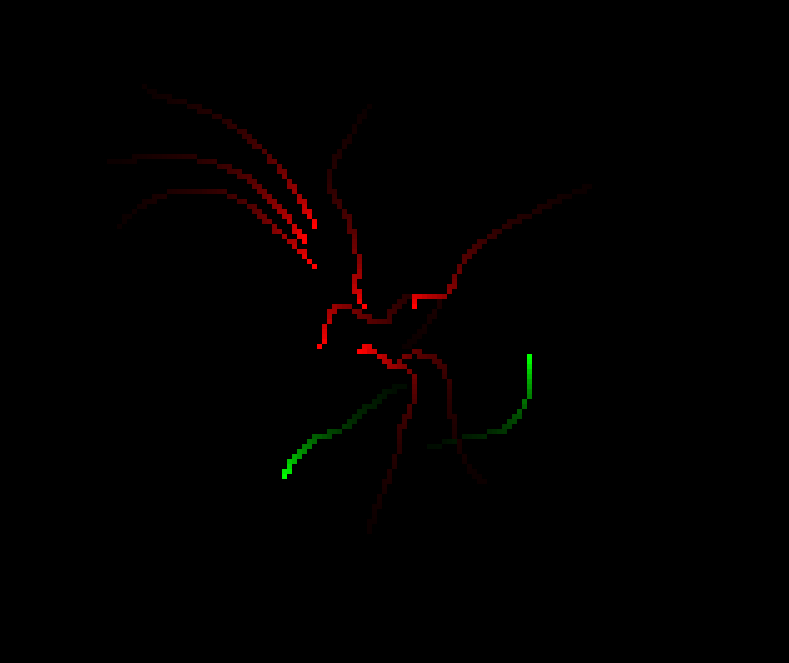
\includegraphics[width=0.3\textwidth]{assets/n8m2_cluster_start.png}
        }
        \subfloat[Tight grouping]{
            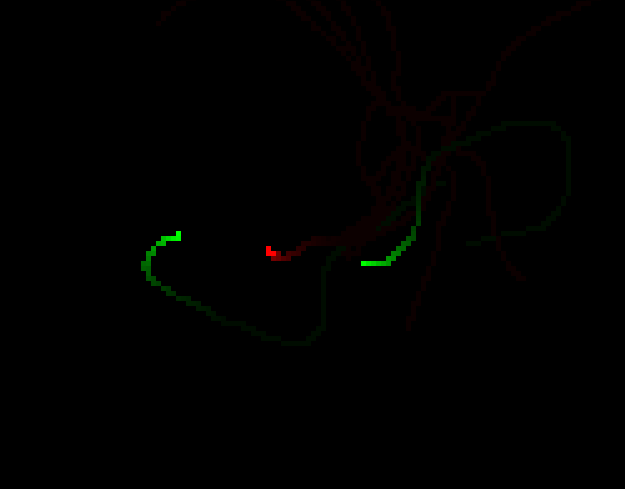
\includegraphics[width=0.3\textwidth]{assets/n8m2_cluster_tight.png}
        }
        \subfloat[Failure to split into full chain]{
            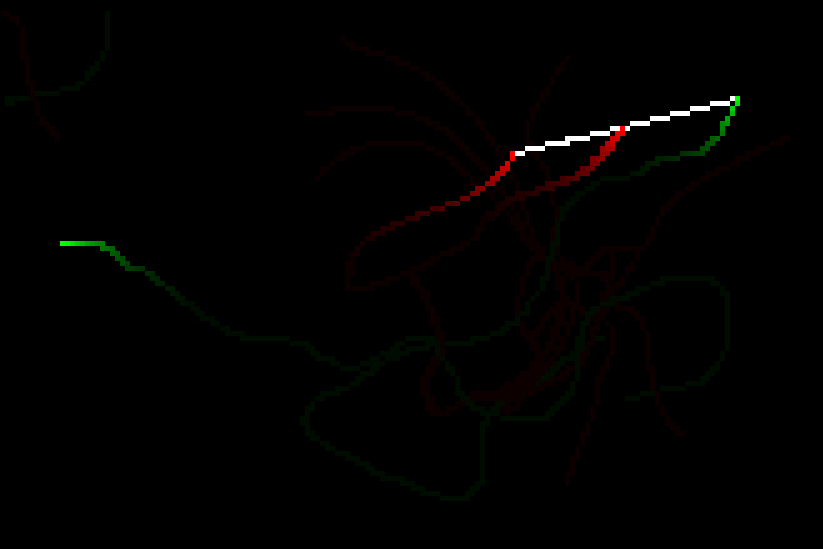
\includegraphics[width=0.3\textwidth]{assets/n8m2_cluster_end.png}
        }
        \caption{Pursuers cluster to maximize connectivity but are reluctant to separate later}
    \end{figure}
\end{frame}

\begin{frame}{Connectivity Analysis}
    \small
    \begin{columns}
        \column{0.5\textwidth}
        \begin{table}
            \begin{tabular}{cccl}
                \hline
                $n$ & $m$ & \% of duration connected & $\bar{\lambda_2}$ \\
                \hline
                1   & 1   & 96.51 \%                 & 1.807             \\
                1   & 2   & 28.48 \%                 & 0.158             \\
                1   & 3   & 11.44 \%                 & 0.041             \\
                2   & 2   & 46.05 \%                 & 0.364             \\
                3   & 3   & 44.97 \%                 & 0.162             \\
                4   & 4   & 40.00 \%                 & 0.191             \\
                5   & 5   & 33.90 \%                 & 0.060             \\
                6   & 1   & 99.69 \%                 & 6.230             \\
                6   & 2   & 64.59 \%                 & 0.923             \\
                6   & 3   & 52.99 \%                 & 0.341             \\
                6   & 4   & 33.18 \%                 & 0.102             \\
                6   & 5   & 33.58 \%                 & 0.083             \\
                6   & 6   & 34.58 \%                 & 0.072             \\
            \end{tabular}
        \end{table}
        \column{0.5\textwidth}
        \begin{table}
            \begin{tabular}{cccl}
                \hline
                $n$ & $m$ & \% of duration connected & $\bar{\lambda_2}$ \\
                \hline
                7   & 3   & 44.69 \%                 & 0.286             \\
                7   & 4   & 42.77 \%                 & 0.156             \\
                7   & 5   & 39.40 \%                 & 0.108             \\
                7   & 6   & 37.69 \%                 & 0.089             \\
                7   & 7   & 35.21 \%                 & 0.060             \\
                8   & 1   & 99.48 \%                 & 7.414             \\
                8   & 2   & 59.04 \%                 & 1.288             \\
                8   & 3   & 44.62 \%                 & 0.307             \\
                8   & 4   & 37.85 \%                 & 0.085             \\
                8   & 5   & 46.72 \%                 & 0.156             \\
                8   & 6   & 32.07 \%                 & 0.084             \\
                8   & 7   & 40.78 \%                 & 0.082             \\
                8   & 8   & 31.16 \%                 & 0.054             \\
            \end{tabular}
        \end{table}
    \end{columns}
    Disconnected at $\lambda_2 \le 10^{-2}$.
\end{frame}

\begin{frame}{Connectivity Analysis}
    \begin{figure}
        \subfloat[$\bar{\lambda_2}$ at each time step for 20 simulations of $n = 6, m = 3$]{
            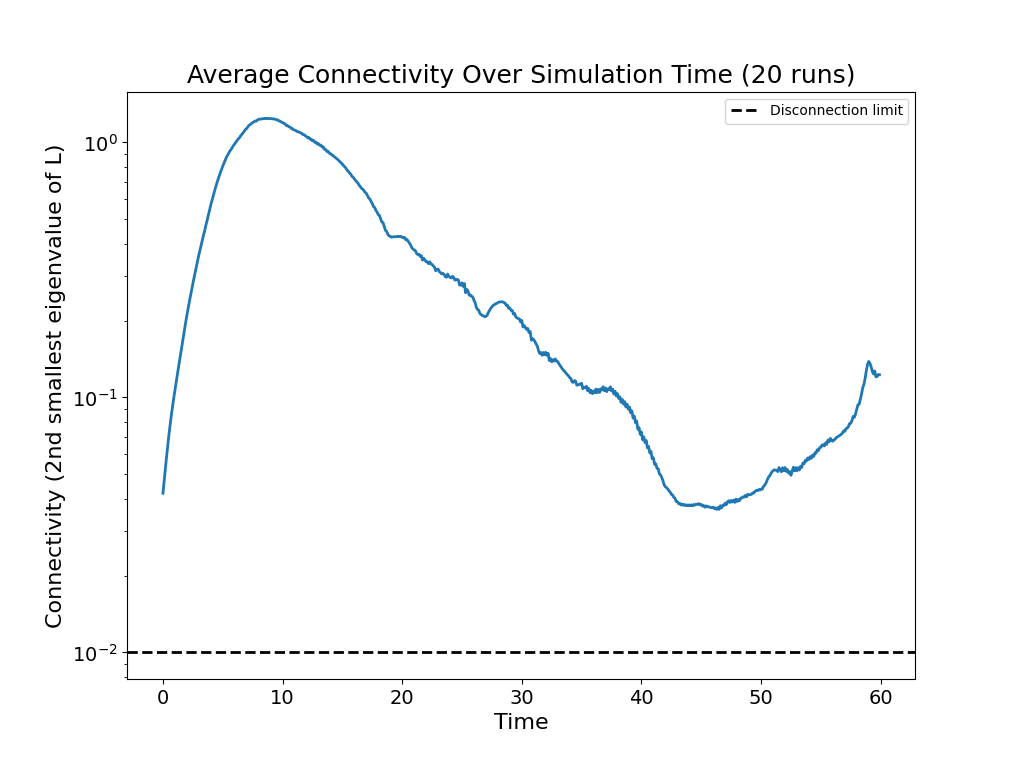
\includegraphics[width=0.45\textwidth]{assets/n6-eig.png}
        }
        \subfloat[$\bar{\lambda_2}$ at each time step for 20 simulations of $n = 8, m = 3$]{
            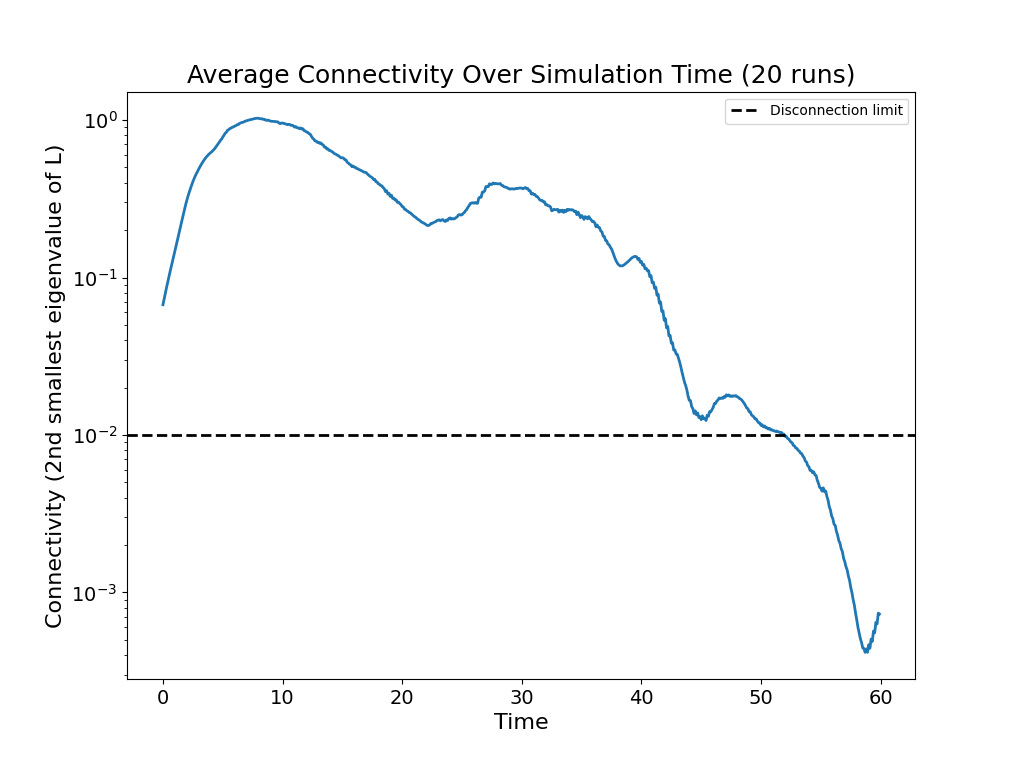
\includegraphics[width=0.45\textwidth]{assets/n8-eig.png}
        }
    \end{figure}
    Grouping behaviour affects connectivity trends. Evaders diffuse out over
    time.
\end{frame}
